\documentclass[border={0pt}, tikz]{standalone}
\usepackage{amsmath}
\usetikzlibrary{bayesnet}

\begin{document}
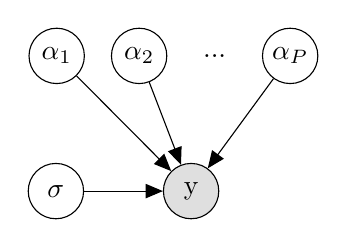
\begin{tikzpicture}
  \node[obs, yshift=1cm] (y) {y};
  
  \node[latent, left=of y] (sigma) {$\sigma$};

  \node[latent, above=of y, xshift=-.66cm] (alpha2) {$\alpha_2$};
  \node[latent, left=.33cm of alpha2] (alpha1) {$\alpha_1$};
  \node[draw=none, right=.33cm of alpha2] (dots) {...};
  \node[latent, right=.33cm of dots] (alphaP) {$\alpha_P$};
  
  \edge {alpha1, alpha2, alphaP, sigma} {y};
\end{tikzpicture}
\end{document}
